\documentclass{standalone}
\usepackage{tikz}
\usetikzlibrary{patterns, positioning}


\begin{document}
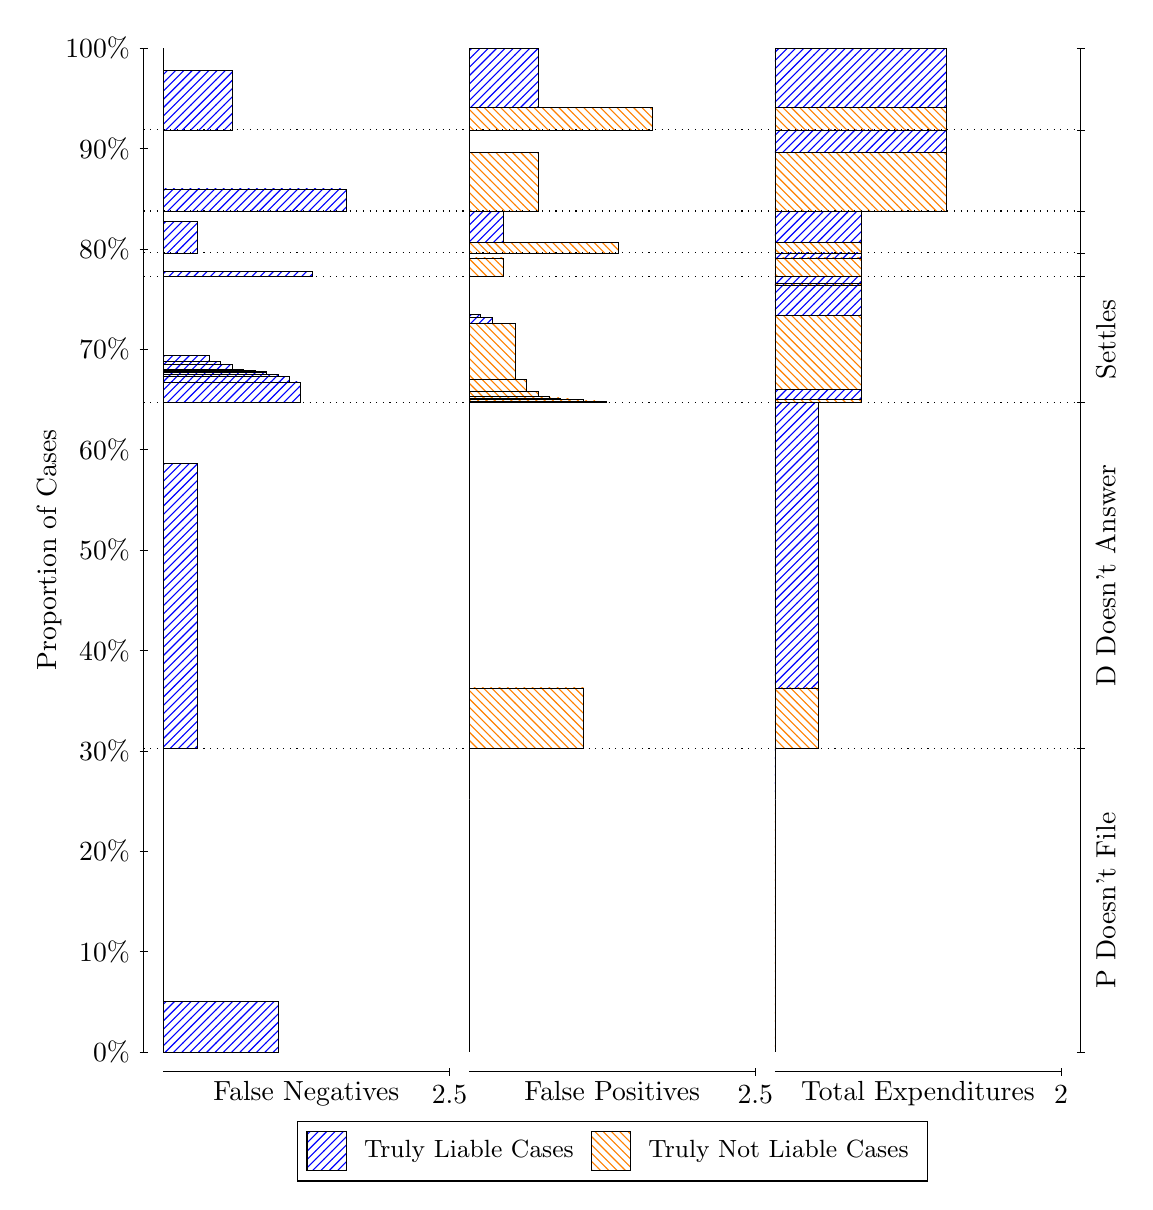
\begin{tikzpicture}
\draw[black, very thin] (1.5,1.75) -- (1.5,14.5);
\node[rotate=90, text=black, anchor=center] at (0.3, 8.125) {Proportion of Cases};
\draw[black, very thin] (1.45,1.75) -- (1.55,1.75);
\node[text=black, anchor=east] at (1.45, 1.75) {0\%};
\draw[black, very thin] (1.45,3.025) -- (1.55,3.025);
\node[text=black, anchor=east] at (1.45, 3.025) {10\%};
\draw[black, very thin] (1.45,4.3) -- (1.55,4.3);
\node[text=black, anchor=east] at (1.45, 4.3) {20\%};
\draw[black, very thin] (1.45,5.575) -- (1.55,5.575);
\node[text=black, anchor=east] at (1.45, 5.575) {30\%};
\draw[black, very thin] (1.45,6.85) -- (1.55,6.85);
\node[text=black, anchor=east] at (1.45, 6.85) {40\%};
\draw[black, very thin] (1.45,8.125) -- (1.55,8.125);
\node[text=black, anchor=east] at (1.45, 8.125) {50\%};
\draw[black, very thin] (1.45,9.4) -- (1.55,9.4);
\node[text=black, anchor=east] at (1.45, 9.4) {60\%};
\draw[black, very thin] (1.45,10.675) -- (1.55,10.675);
\node[text=black, anchor=east] at (1.45, 10.675) {70\%};
\draw[black, very thin] (1.45,11.95) -- (1.55,11.95);
\node[text=black, anchor=east] at (1.45, 11.95) {80\%};
\draw[black, very thin] (1.45,13.225) -- (1.55,13.225);
\node[text=black, anchor=east] at (1.45, 13.225) {90\%};
\draw[black, very thin] (1.45,14.5) -- (1.55,14.5);
\node[text=black, anchor=east] at (1.45, 14.5) {100\%};

\draw[black, very thin] (13.4,1.75) -- (13.4,14.5);
\draw[black, very thin] (13.35,1.75) -- (13.45,1.75);
\node[anchor=west] at (13.35, 1.75) {};
\draw[black, very thin] (13.35,5.6007) -- (13.45,5.6007);
\node[anchor=west] at (13.35, 5.6007) {};
\draw[black, very thin] (13.35,10.001) -- (13.45,10.001);
\node[anchor=west] at (13.35, 10.001) {};
\draw[black, very thin] (13.35,11.602) -- (13.45,11.602);
\node[anchor=west] at (13.35, 11.602) {};
\draw[black, very thin] (13.35,11.899) -- (13.45,11.899);
\node[anchor=west] at (13.35, 11.899) {};
\draw[black, very thin] (13.35,12.43) -- (13.45,12.43);
\node[anchor=west] at (13.35, 12.43) {};
\draw[black, very thin] (13.35,13.461) -- (13.45,13.461);
\node[anchor=west] at (13.35, 13.461) {};
\draw[black, very thin] (13.35,14.5) -- (13.45,14.5);
\node[anchor=west] at (13.35, 14.5) {};

\draw[black, very thin, pattern color=blue, pattern=north east lines] (1.75,1.75) rectangle (3.2033,2.3971);
\draw[black, very thin, pattern color=orange, pattern=north west lines] (1.75,2.3971) rectangle (1.75,5.6007);
\draw[black, very thin, pattern color=blue, pattern=north east lines] (1.75,5.6007) rectangle (2.186,9.2278);
\draw[black, very thin, pattern color=orange, pattern=north west lines] (1.75,9.2278) rectangle (1.75,10.001);
\draw[black, very thin, pattern color=blue, pattern=north east lines] (1.75,10.001) rectangle (3.494,10.259);
\draw[black, very thin, pattern color=blue, pattern=north east lines] (1.75,10.259) rectangle (3.3487,10.325);
\draw[black, very thin, pattern color=blue, pattern=north east lines] (1.75,10.325) rectangle (3.2033,10.357);
\draw[black, very thin, pattern color=blue, pattern=north east lines] (1.75,10.357) rectangle (3.058,10.385);
\draw[black, very thin, pattern color=blue, pattern=north east lines] (1.75,10.385) rectangle (3.058,10.389);
\draw[black, very thin, pattern color=blue, pattern=north east lines] (1.75,10.389) rectangle (2.9127,10.411);
\draw[black, very thin, pattern color=blue, pattern=north east lines] (1.75,10.411) rectangle (2.7673,10.418);
\draw[black, very thin, pattern color=blue, pattern=north east lines] (1.75,10.418) rectangle (2.622,10.483);
\draw[black, very thin, pattern color=blue, pattern=north east lines] (1.75,10.483) rectangle (2.4767,10.518);
\draw[black, very thin, pattern color=blue, pattern=north east lines] (1.75,10.518) rectangle (2.3313,10.601);
\draw[black, very thin, pattern color=orange, pattern=north west lines] (1.75,10.601) rectangle (1.75,11.602);
\draw[black, very thin, pattern color=blue, pattern=north east lines] (1.75,11.602) rectangle (3.6393,11.667);
\draw[black, very thin, pattern color=orange, pattern=north west lines] (1.75,11.667) rectangle (1.75,11.899);
\draw[black, very thin, pattern color=blue, pattern=north east lines] (1.75,11.899) rectangle (2.186,12.296);
\draw[black, very thin, pattern color=orange, pattern=north west lines] (1.75,12.296) rectangle (1.75,12.43);
\draw[black, very thin, pattern color=blue, pattern=north east lines] (1.75,12.43) rectangle (4.0753,12.712);
\draw[black, very thin, pattern color=orange, pattern=north west lines] (1.75,12.712) rectangle (1.75,13.461);
\draw[black, very thin, pattern color=blue, pattern=north east lines] (1.75,13.461) rectangle (2.622,14.217);
\draw[black, very thin, pattern color=orange, pattern=north west lines] (1.75,14.217) rectangle (1.75,14.5);
\draw[black, very thin, pattern color=orange, pattern=north west lines] (5.6333,1.75) rectangle (5.6333,4.9536);
\draw[black, very thin, pattern color=blue, pattern=north east lines] (5.6333,4.9536) rectangle (5.6333,5.6007);
\draw[black, very thin, pattern color=orange, pattern=north west lines] (5.6333,5.6007) rectangle (7.0867,6.3737);
\draw[black, very thin, pattern color=blue, pattern=north east lines] (5.6333,6.3737) rectangle (5.6333,10.001);
\draw[black, very thin, pattern color=orange, pattern=north west lines] (5.6333,10.001) rectangle (7.3773,10.012);
\draw[black, very thin, pattern color=orange, pattern=north west lines] (5.6333,10.012) rectangle (7.232,10.019);
\draw[black, very thin, pattern color=orange, pattern=north west lines] (5.6333,10.019) rectangle (7.0867,10.038);
\draw[black, very thin, pattern color=orange, pattern=north west lines] (5.6333,10.038) rectangle (6.9413,10.043);
\draw[black, very thin, pattern color=orange, pattern=north west lines] (5.6333,10.043) rectangle (6.796,10.057);
\draw[black, very thin, pattern color=orange, pattern=north west lines] (5.6333,10.057) rectangle (6.6507,10.08);
\draw[black, very thin, pattern color=orange, pattern=north west lines] (5.6333,10.08) rectangle (6.5053,10.143);
\draw[black, very thin, pattern color=orange, pattern=north west lines] (5.6333,10.143) rectangle (6.36,10.295);
\draw[black, very thin, pattern color=orange, pattern=north west lines] (5.6333,10.295) rectangle (6.2147,11.002);
\draw[black, very thin, pattern color=blue, pattern=north east lines] (5.6333,11.002) rectangle (5.924,11.084);
\draw[black, very thin, pattern color=blue, pattern=north east lines] (5.6333,11.084) rectangle (5.7787,11.12);
\draw[black, very thin, pattern color=blue, pattern=north east lines] (5.6333,11.12) rectangle (5.6333,11.602);
\draw[black, very thin, pattern color=orange, pattern=north west lines] (5.6333,11.602) rectangle (6.0693,11.835);
\draw[black, very thin, pattern color=blue, pattern=north east lines] (5.6333,11.835) rectangle (5.6333,11.899);
\draw[black, very thin, pattern color=orange, pattern=north west lines] (5.6333,11.899) rectangle (7.5227,12.033);
\draw[black, very thin, pattern color=blue, pattern=north east lines] (5.6333,12.033) rectangle (6.0693,12.43);
\draw[black, very thin, pattern color=orange, pattern=north west lines] (5.6333,12.43) rectangle (6.5053,13.178);
\draw[black, very thin, pattern color=blue, pattern=north east lines] (5.6333,13.178) rectangle (5.6333,13.461);
\draw[black, very thin, pattern color=orange, pattern=north west lines] (5.6333,13.461) rectangle (7.9587,13.743);
\draw[black, very thin, pattern color=blue, pattern=north east lines] (5.6333,13.743) rectangle (6.5053,14.5);
\draw[black, very thin, pattern color=orange, pattern=north west lines] (9.5167,1.75) rectangle (9.5167,4.9536);
\draw[black, very thin, pattern color=blue, pattern=north east lines] (9.5167,4.9536) rectangle (9.5167,5.6007);
\draw[black, very thin, pattern color=orange, pattern=north west lines] (9.5167,5.6007) rectangle (10.062,6.3737);
\draw[black, very thin, pattern color=blue, pattern=north east lines] (9.5167,6.3737) rectangle (10.062,10.001);
\draw[black, very thin, pattern color=orange, pattern=north west lines] (9.5167,10.001) rectangle (10.607,10.041);
\draw[black, very thin, pattern color=blue, pattern=north east lines] (9.5167,10.041) rectangle (10.607,10.164);
\draw[black, very thin, pattern color=orange, pattern=north west lines] (9.5167,10.164) rectangle (10.607,11.107);
\draw[black, very thin, pattern color=blue, pattern=north east lines] (9.5167,11.107) rectangle (10.607,11.491);
\draw[black, very thin, pattern color=orange, pattern=north west lines] (9.5167,11.491) rectangle (10.607,11.509);
\draw[black, very thin, pattern color=blue, pattern=north east lines] (9.5167,11.509) rectangle (10.607,11.602);
\draw[black, very thin, pattern color=orange, pattern=north west lines] (9.5167,11.602) rectangle (10.607,11.835);
\draw[black, very thin, pattern color=blue, pattern=north east lines] (9.5167,11.835) rectangle (10.607,11.899);
\draw[black, very thin, pattern color=orange, pattern=north west lines] (9.5167,11.899) rectangle (10.607,12.033);
\draw[black, very thin, pattern color=blue, pattern=north east lines] (9.5167,12.033) rectangle (10.607,12.43);
\draw[black, very thin, pattern color=orange, pattern=north west lines] (9.5167,12.43) rectangle (11.697,13.178);
\draw[black, very thin, pattern color=blue, pattern=north east lines] (9.5167,13.178) rectangle (11.697,13.461);
\draw[black, very thin, pattern color=orange, pattern=north west lines] (9.5167,13.461) rectangle (11.697,13.743);
\draw[black, very thin, pattern color=blue, pattern=north east lines] (9.5167,13.743) rectangle (11.697,14.5);
\draw[black, dotted] (1.5,5.6007) -- (13.4,5.6007);
\draw[black, dotted] (1.5,10.001) -- (13.4,10.001);
\draw[black, dotted] (1.5,11.602) -- (13.4,11.602);
\draw[black, dotted] (1.5,11.899) -- (13.4,11.899);
\draw[black, dotted] (1.5,12.43) -- (13.4,12.43);
\draw[black, dotted] (1.5,13.461) -- (13.4,13.461);
\draw[black, very thin] (1.75,1.5) -- (5.3833,1.5);
\node[text=black, anchor=north] at (3.5667, 1.5) {False Negatives};
\draw[black, very thin] (5.3833,1.45) -- (5.3833,1.55);
\node[text=black, anchor=north] at (5.3833, 1.45) {2.5};

\draw[black, very thin] (5.6333,1.5) -- (9.2667,1.5);
\node[text=black, anchor=north] at (7.45, 1.5) {False Positives};
\draw[black, very thin] (9.2667,1.45) -- (9.2667,1.55);
\node[text=black, anchor=north] at (9.2667, 1.45) {2.5};

\draw[black, very thin] (9.5167,1.5) -- (13.15,1.5);
\node[text=black, anchor=north] at (11.333, 1.5) {Total Expenditures};
\draw[black, very thin] (13.15,1.45) -- (13.15,1.55);
\node[text=black, anchor=north] at (13.15, 1.45) {2};

\node[text=black, centered, rotate=90] at (13.72, 3.6753) {P Doesn't File};
\node[text=black, centered, rotate=90] at (13.72, 7.8008) {D Doesn't Answer};
\node[text=black, centered, rotate=90] at (13.72, 10.801) {Settles};





\draw (7.449999999999999,1.5) node[draw=none] (baseCoordinate) {};
\begin{scope}[align=center]
        \matrix[scale=0.5, draw=black, below=0.5cm of baseCoordinate, nodes={draw}, column sep=0.1cm]{
            \node[rectangle, draw, minimum width=0.5cm, minimum height=0.5cm, pattern color=blue, pattern=north east lines] {}; &
            \node[draw=none, font=\small, text=black] (B) {Truly Liable Cases}; &
            \node[rectangle, draw, minimum width=0.5cm, minimum height=0.5cm, pattern color=orange, pattern=north west lines] {}; &
            \node[draw=none, font=\small, text=black] (B) {Truly Not Liable Cases}; \\
            };
\end{scope}

\end{tikzpicture}
\end{document}